\documentclass[12pt,UTF8]{ctexart}
\usepackage{ctex,amsmath,amssymb,geometry,fancyhdr,bm,amsfonts
,mathtools,extarrows,graphicx,enumerate,indentfirst,url,float,multicol,subfig} 
% 加入中文支持
\newcommand\Set[2]{%
\left\{#1\ \middle\vert\ #2 \right\}}
\geometry{a4paper,scale=0.80}
\pagestyle{fancy}
\rhead{习题1.2\&1.3\&1.4}
\lhead{基础习题课讲义}
\chead{微积分B(1)}
%\pagestyle{fancy}
%\rhead{习题1.2}
%\lhead{基础习题课讲义}
%\chead{微积分B(1)}
\begin{document}
\setcounter{section}{0}
\section{实数与函数}
\noindent
\subsection{有关说明}
\begin{itemize}
\item 基础习题课时间: 周一第六大节, 地点: 五教5105
\item 基础习题课答疑时间: 周二下午四点到五点, 地点: 理科楼B201
\item 基础习题课助教: 赵东阳, 电话: 18811708556, 邮箱: dy-zhao14@mails.tsinghua.edu.cn, 微信: 18811708556
\item 基础习题课的教学目标:
	\begin{itemize}
		\item使同学掌握课程基本内容
		\item使同学掌握常见问题的一般解法
		\item使同学学会正确地书写解答过程
	\end{itemize}
\item 其他要求和说明:
	\begin{itemize}
		\item每次课前都要签到
		\item上课的同学可以加入基础习题课微信群
		\item基础习题课都非常基础, 注重一般解法和解答过程的书写, 主要面向高年级的同学和一年级的基础相对薄弱的同学, 如果觉得题目简单可有选择地自愿参加
		\item本人是第一次做微积分助教, 还处在一个探索的阶段, 有些问题可能会解释不清楚, 有些环节的安排可能会不太合理. 大家如果觉得听不懂, 或者觉得什么环节安排得不合理, 可以在课下直接指出. 或者可以给我打电话, 发短信, 发邮件. 也可以加我微信
	\end{itemize}
\end{itemize}
\subsection{实数和实数集}
\subsubsection{知识结构}
\noindent第一章 实数与函数
\begin{enumerate}
\item[1.1] 集合与符号
	\begin{enumerate}
		\item[1.1.1] 集合的概念和运算
		\item[1.1.2] 邻域
		\item[1.1.3] 符号“$\forall$”与“$\exists$”
	\end{enumerate}
\item[1.2] 实数和实数集
	\begin{enumerate}
		\item[1.2.1] 实数
			\begin{enumerate}
				\item[1.]数轴
				\item[2.]有理数和无理数
					\begin{itemize}
						\item有理数在实数中的稠密性
					\end{itemize}
			\end{enumerate}
		\item[1.2.2] 实数集的界与确界
			\begin{itemize}
				\item集合有界的充分必要条件
				\item确界存在性定理1.2.2
				\item确界的充分必要条件, 定理1.2.3
				\item确界与最值的关系
			\end{itemize}
	\end{enumerate}
\end{enumerate}
\subsubsection{定理1.2.3的证明}
\noindent{\bf定理1.2.3}  设$E$为非空集合, $a,b$为实数. 则有
\indent
\begin{enumerate}
\item[(1)]b=sup$E$的充分必要条件是下列两个条件同时满足:
	\begin{enumerate}
		\item[\textcircled{1}]$b$是$E$的一个上界;
		\item[\textcircled{2}]对于任意满足$c<b$的实数$c$, $\exists x\in E$, 使得$x>c$.
	\end{enumerate}
\item[(2)]b=inf$E$的充分必要条件是下列两个条件同时满足:
	\begin{enumerate}
		\item[\textcircled{1}]$a$是$E$的一个下界;
		\item[\textcircled{2}]对于任意满足$c>a$的实数$c$, $\exists x\in E$, 使得$x<c$.
	\end{enumerate}
\end{enumerate}
{\bf证明:}
(1)必要性: 设b=sup$E$. 根据定义, $b$必然是$E$的一个上界. 其次, 由于b=sup$E$是集合$E$的最小上界, 所以当$c<b$时, $c$不是集合$E$的上界. 于是至少存在一个$x\in E$, 使得$x>c$.
\newline
充分性: $b$是集合$E$的一个上界. 为了证明b=sup$E$, 只需要证明: 当$c<b$时, $c$都不是$E$的上界. 而这一点可以由条件$\textcircled2$推出.
\newline
(2)必要性: 设a=inf$E$. 根据定义, $a$必然是$E$的一个下界. 其次, 由于a=inf$E$是集合$E$的最大下界, 所以当$c>a$时, $c$不是集合$E$的下界. 于是至少存在一个$x\in E$, 使得$x<c$.
\newline
充分性: $a$是集合$E$的一个下界. 为了证明a=inf$E$, 只需要证明: 当$c>a$时, $c$都不是$E$的下界. 而这一点可以由条件$\textcircled2$推出.
\newline
{\bf(数轴图示.)}
\newline
{\bf(提醒学生注意记住定理,通过训练牢固掌握定理,要像加减乘除四则运算和运算律一样灵活使用,不必纠结于证明过程,重要的是应用,要用直观的方法记住.)}\footnotemark[1]\footnotetext[1]{字体加粗的内容会在课上讲解或者提到.}
\subsubsection{习题1.2解答}
\begin{enumerate}
\item 
对于实数集A,supA(infA)与maxA(minA)有什么联系和区别?下列集合中哪些有上、下确界和最大、最小值?
\begin{enumerate}
\item[(1)]自然数集$\mathbb Z^+$;
\item[(2)]$(0,1)$中所有有理数;
\item[(3)]有限个数构成的集合$\{a_1,a_2,\dots,a_n\}$;
\item[\bf(4)]\footnotemark[2]\footnotetext[2]{序号加粗的题目会在课上讲解.}$\{x\in \mathbb{R}|\text{x为有理数,且}x^2<2\}$;
\item[\bf(5)]$[0,1]$与$(0,1)$;
\item[(6)]$\{x\in\mathbb{R}|x^2-2x-3<0\},\{x\in\mathbb{R}|x^2-2x-3\leq0\}$.
\end{enumerate}
解答:supA(infA)与maxA(minA)之间的关系可以概括为以下两点:
\newline(i)如果非空集合A有上(下)界,则必存在supA(infA),但未必存在maxA(minA),比如$(0,1)$;
\newline(ii)如果非空集合A存在maxA(minA),则supA=maxA(infA=minA).
\begin{enumerate}
\item[(1)]不存在上确界和最大值,inf$\mathbb Z^+$=min$\mathbb Z^+$=1.
\item[(2)]下确界为0,上确界为1,无最大最小值.
\item[(3)]上确界和最大值为max$\{a_1,a_2,\dots,a_n\}$,下确界和最小值为min$\{a_1,a_2,\dots,a_n\}$.
\item[\bf(4)]上确界为$\sqrt2$, 下确界为$-\sqrt2$, 无最大和最小值. 这里$\{x\in \mathbb{R}|\text{x为有理数,且}x^2<2\}\Leftrightarrow\{x\in \mathbb{R}|\text{x为有理数, 且}x\in(-\sqrt2,\sqrt2)\}$, 因此$\pm\sqrt2$为原集合的上下界. $\forall c<\sqrt2,\exists\text{有理数}x>c$, 根据定理1.2.3, $\sqrt2$是原集合的上界. $\forall c>-\sqrt2,\exists\text{有理数}x<c$, 根据定理1.2.3, $-\sqrt2$是原集合的下界(或者同理可得$-\sqrt2$是原集合的下界). 假设存在最大值A, 则$A\in\mathbb Q$, 则$A<\sqrt2$, 则由有理数集的稠密性, 在A和$\sqrt2$之间存在无穷多个有理数, 这与A是最大值矛盾, 故原集合不存在最大值. 同理, 原集合也不存在最小值.
\item[\bf(5)]$[0,1]$的最大值为1, 则上确界也为1, 最小值为0, 则下确界为0.  $(0,1)$的上确界为1, 下确界为0, 不存在最大和最小值. 这里, 由1(0)是$(0,1)$的上(下)界, 且$\forall c<1(>0),\ \exists x\in(0,1),\ x>(<)c$, 根据定理1.2.3可知, 1(0)分别是$(0,1)$的上(下)确界. 假设A是$(0,1)$的最大(小)值, 则$A<1(>0)$, 在A和1(0)之间存在无穷多个实数, 与A是$(0,1)$的最大(小)值矛盾, 故$(0,1)$不存在最大和最小值.
\item[(6)]$\{x\in\mathbb{R}|x^2-2x-3<0\}\Leftrightarrow(-2,3)$,其上确界是3,下确界是-2,不存在最大最小值,$\{x\in\mathbb{R}|x^2-2x-3\leq0\}\Leftrightarrow[-2,3]$,其最大值是3,则上确界为3,最小值是-2,则下确界是-2.
\end{enumerate}
\item[\bf2.]设$a_1,a_2,\dots,a_n,\dots$是一列实数, A是一个确定的实数, $\forall\varepsilon>0$, 令$G_\varepsilon=\{n\in\mathbb Z^+||a_n-A|<\varepsilon\}$.
\begin{enumerate}
\item[\bf(1)]若$0<\varepsilon_1<\varepsilon_2$,求证$G_{\varepsilon_1}\subseteq G_{\varepsilon_2}$;
\item[\bf(2)]$\bigcup\limits_{\varepsilon>0}G_{\varepsilon}$是什么集合?
\item[\bf(3)]$\bigcap\limits_{\varepsilon>0}G_{\varepsilon}$何时非空?
\end{enumerate}
其中$\bigcup\limits_{\varepsilon>0}G_{\varepsilon}$表示所有集合$G_{\varepsilon}(\varepsilon>0)$的并集与交集.
\newline
解答:\begin{enumerate}
\item[\bf(1)]{\bf(思路: 先观察集合$G_\varepsilon$, 是一个整数集的子集, 满足一定的条件, 从该条件出发, 构造集合$\bar{G}_\varepsilon=\{a_n|n\in G_\varepsilon\}=\{x|x\in\{a_1,a_2,\dots,a_n,\dots\},|x-A|<\varepsilon\}$, 容易证明$\bar{G}_{\varepsilon_1}\subseteq \bar{G}_{\varepsilon_2}$, 将证明过程中的$x$换为$a_n$即可.)}
\newline证明: $\forall n\in G_{\varepsilon_1},\ |a_n-A|<\varepsilon_1,\ A-\varepsilon_1<a_n<A+\varepsilon_1,\ \because 0<\varepsilon_1<\varepsilon_2,\ \therefore A-\varepsilon_2<a_n<A+\varepsilon_2,\ \therefore |a_n-A|<\varepsilon_2,\ \therefore n\in G_{\varepsilon_2},\ \therefore G_{\varepsilon_1}\subseteq G_{\varepsilon_2}$, 证毕.
\item[\bf(2)]$\mathbb Z^+$. {\bf(思路: 当$\varepsilon\rightarrow\infty,\ \bar{G}_\varepsilon=\{a_1,a_2,\dots,a_n,\dots\}$, 即当$\varepsilon$足够大时, $A$的$\varepsilon$邻域可包含$\{a_1,a_2,\dots,a_n,\dots\}$, 此时$G_\varepsilon=\mathbb Z^+$. 注意等号的位置.)}
\newline
证明: 令M=max$\{|a_1-A|,|a_2-A|,\dots,|a_n-A|,\dots\},\ \forall\varepsilon_M>M,\ \bar{G}_{\varepsilon_M}=\{x|x\in\{a_1,a_2,\dots,a_n,\dots\},\ |x-A|<\varepsilon\}=\{a_1,a_2,\dots,a_n,\dots\},\ \therefore G _{\varepsilon_M}=\{n\in\mathbb Z^+||a_n-A|<\varepsilon\}=\mathbb{Z}^+,\ \text{由(1)知}\forall0<\varepsilon\leq M<\varepsilon_M, \ G_{\varepsilon}\subseteq G_{\varepsilon_M}=\mathbb{Z}^+,\ \therefore\bigcup\limits_{\varepsilon>0}G_{\varepsilon}=\mathbb{Z}^+$, 证毕.
\item[\bf(3)]要使$\bigcap\limits_{\varepsilon>0}G_{\varepsilon}$非空, 则$\forall\varepsilon>0$, $G_{\varepsilon}$非空, 且$\varepsilon\rightarrow0$时, 最小的集合$G_{\varepsilon}$非空. 则要求$\exists n\in\mathbb{Z}^+,\ |a_n-A|=0$, 即$\exists n\in\mathbb{Z}^+,\ a_n=A$.
\end{enumerate}
\item[\bf3.] 设$S=\{x\in\mathbb R|x^2<2\}$,求证supS=$\sqrt2$.
\newline
{\bf(定理1.2.3的应用)}
\newline
证明: $S=\{x\in\mathbb R|x^2<2\}=(-\sqrt2,\sqrt2),\ \therefore\forall x\in S, x<\sqrt2$, 故$\sqrt2$是S的上界. $\forall c<\sqrt2, \ \exists x\in(c,\sqrt2), x>c$(满足定理1.2.3的第二个条件), 故supS=$\sqrt2$.
\item[4.] 若A,B为$\mathbb R$中的非空有界集,则A$\cup$B与A$\cap$B也是有界集,并且
\newline
inf(A$\cup$B)=min\{infA,infB\},\ sup(A$\cup$B)=max\{supA,supB\},
\newline
inf(A$\cap$B)$\geq$max\{infA,infB\},\ sup(A$\cap$B)$\leq$min\{supA,supB\}.
\newline
(后面两式仅当A$\cap$B$\neq\emptyset$时成立)
\newline
{\bf(证明过程比较繁琐,但还是定理1.2.3的应用.)}
\newline
证明:$\because A,B$为$\mathbb R$中的非空有界集,$\therefore A,B$有上下确界,$\therefore \forall a\in A,\ {\rm inf}A\leq a\leq{\rm sup}A,\ \forall b\in B,\ \rm{inf}B\leq b\leq\rm{sup}B,\ \therefore\forall c\in A\cup B,\ {\rm min}\{{\rm inf}A,{\rm inf}B\}\leq c\leq{\rm max}\{{\rm inf}A,{\rm inf}B\},\ \forall d\in A\cap B,\ {\rm max}\{{\rm inf}A,{\rm inf}B\}\leq d\leq{\rm min}\{{\rm inf}A,{\rm inf}B\},\ \therefore A\cup B,A\cap B$均为有界集.
\newline
$\forall e>{\rm min}\{{\rm inf}A,{\rm inf}B\},\ \exists x\in A\text{或}B,\ x<e$,故inf(A$\cup$B)=min\{infA,infB\}.同理,sup(A$\cup$B)
=max\{supA,supB\}.
\newline
max\{infA,infB\}是$A\cap B$的下界但非下确界,即$\exists f>$max\{infA,infB\}, $\forall x\in A\cap B,\ x>f$,如$A=\{0,2,3,4\},B=\{1,2,3,5\},$infA=0,infB=1,但A$\cap$B=\{2,3\},inf(A$\cap$B)=2$>$
\newline 
max\{infA,infB\},故inf(A$\cap$B)$\geq$max\{infA,infB\}.同理,sup(A$\cap$B)$\leq$min\{supA,supB\}.
\item[5.]设a,b为任意的两个实数,求证:
\newline
${\rm max}\{a,b\}=\frac{a+b+|a-b|}2,\ {\rm min}\{a,b\}=\frac{a+b-|a-b|}2$.
\newline
{\bf(可从要证的结论出发反推出已知条件.)}
\newline
证明:$\because {\rm max}\{a,b\}+{\rm min}\{a,b\}=a+b,\ {\rm max}\{a,b\}-{\rm min}\{a,b\}=|a-b|,\therefore {\rm max}\{a,b\}=\frac{a+b+|a-b|}2,\ {\rm min}\{a,b\}=\frac{a+b-|a-b|}2$
\end{enumerate}

\subsection{函数}
\noindent
\subsubsection{知识结构}
\noindent第一章实数与函数
	\begin{enumerate}
		\item[1.1] 集合与符号
		\item[1.2] 实数和实数集
		\item[1.3] 函数
			\begin{enumerate}
				\item[1.3.1] 函数概念
				\item[1.3.2] 函数的一些重要属性
					\begin{enumerate}
						\item[1.] 奇偶性
						\item[2.] 单调性
						\item[3.] 周期性
						\item[4.] 有界性
					\end{enumerate}
               \item[1.3.3] 反函数与复合函数
               	\begin{enumerate}
               		\item[1.] 反函数
               		\item[2.] 复合函数
               	\end{enumerate}
				\item[1.3.4] 函数的平移和伸缩
				\item[1.3.5] 映射
					\begin{itemize}
						\item 单射
						\item 满射
						\item 双射
						\item 逆映射
					\end{itemize}
			\end{enumerate}
	\end{enumerate}
\subsubsection{重点内容}
\begin{enumerate}
   \item 周期性(习题3、8)
   \item 有界性(习题7)
   \item 函数的平移和伸缩(习题9、12)
   		\begin{itemize}
			\item 口诀: 左加右减, 上加下减; 对于x, 大于1缩小, 小于1放大;  对于y, 大于1放大, 小于1缩小
			\item 直观理解$a>0, f(\underline x),\ f(\underline{x+a}),\ f(\underline{x-a}),\ f(\underline{ax}),\ f(x)+a,\ f(x)-a$
			\item 先伸缩, 后平移
		\end{itemize}
   \item 映射(习题11、12)
   		\begin{itemize}
			\item 单射、满射、双射的图示
		\end{itemize}
   \item 反证法(习题4)
\end{enumerate}
\subsubsection{习题1.3解答}
\begin{enumerate}
\item 设$f(x)=\begin{cases}x+1,&x\geq0\\0,&x<0\end{cases},g(x)=\begin{cases}0,&x>0\\2,&x\leq0\end{cases},$求$f\circ g$与$g\circ f$,验证是否有$f\circ g=g\circ f$.
\newline
{\bf(函数复合不具有交换律.)}
\newline
解:$f\circ g(x)=f(g(x))=\begin{cases}1,&x>0\\3,&x\leq0\end{cases},g\circ f(x)=g(f(x))=\begin{cases}0,&x\geq0\\2,&x<0\end{cases}$.$f\circ g\neq g\circ f$.
\item 已知$f(x+1)=2x^2-x+1,\ g(x+\frac1x)=x^2+\frac1{x^2}(x\neq0)$,写出$f(x),g(x)$的表达式.
\newline
{\bf(技巧.)}
\newline
解:$f(x+1)=2x^2-x+1$中,令$t=x+1$,则$x=t-1$,$f(t)=2(t-1)^2-(t-1)+1=2t^2-5t+4$,即$f(x)=2x^2-5x+4$.
\newline
$g(x+\frac1x)=x^2+\frac1{x^2}=(x+\frac1x)^2-2$,则$g(x)=x^2-2$.
\item[\bf3.] 设$f(x)$是以2为周期的奇函数,并且当$0\leq x\leq1$时,$f(x)=x(1-x)$.试写出$f(x)$的表达式,并画出图像.
\newline
{\bf(先给出$(-1,0)$上的表达式, 得到一个周期内的表达式, 再扩展到整个$(-\infty,+\infty)$. 严格起见, 区间端点处的等号不重复加.)}
\newline
解: 当$-1\leq x<0$时, $f(x)=-f(-x)=-(-x)[1-(-x)]=x(1+x)$, 则
\[
f(x)=\begin{cases}
(x-2n)[1+(x-2n)],&-1+2n\leq x<2n\\
(x-2n)[1-(x-2n)],&2n\leq x<1+2n
\end{cases},\ n\in\mathbb Z
\]
\begin{figure}[H]
\begin{center}
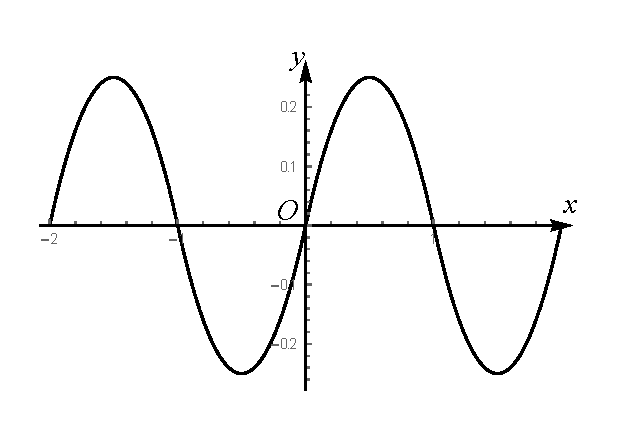
\includegraphics[height=0.3\textheight]{F:/life/2018AutumnTA/Exercises/1/problem3.pdf}
\end{center}
\caption{3.题$f(x)$的图像}
\end{figure}
\item[\bf4.] 设$f(x)$是定义在$(-\infty,+\infty)$上的函数,并且满足$f(2x)=2f(x)$. 试证: 如果$f$在$(-\infty,+\infty)$上有界, 则$f(x)\equiv0$.
\newline
{\bf(反证法. 要证明恒等于0, 只需证明不等于0的$f(x)$不存在, 于是假设存在等于0的点, 推出矛盾.)}
\newline
证明: $\because f(x)$在$(-\infty,+\infty)$上有界, $\therefore\exists M>0,\ \forall x\in(-\infty,+\infty),\ |f(x)|<M$.
\newline
假设$f(x_0)=A\neq0$, 则由$f(2x)=2f(x)$可知$f(2x_0)=2A,f(4x_0)=4A,\dots,f(2^nx_0)=2^nA,\dots,n\in\mathbb Z^+${\bf($|2^nA|$一定会大于$M$, 可解出满足条件的$n$.)}, 取$n>\log_2\frac M{|A|}$, 则$|f(x)|>M$, 矛盾. 故$f(x)\equiv0$.
\item[\bf5.]两个单调增加的函数的复合函数是否一定单调增加? 它们的乘积又如何? 
\newline
{\bf(一定需要证明, 不一定只需给出反例.)}
\newline
解: 两个单调增加的函数的复合函数一定单调增加, 但二者的乘积不一定单调增加. 设这两个函数分别为$f(x),g(x)$, 对于$x_1<x_2$, 有$g(x_1)<g(x_2)$, 则$f(g(x_1))<f(g(x_2))$, 所以$f\circ g(x)$单调增加. 若$f(x_1)=-2,f(x_2)=-1,g(x_1)=1,g(x_2)=3$, 则$f(x_1)g(x_1)=-2>-3=f(x_2)g(x_2)$, 此时$f(x)g(x)$不单调增加.
\item[6.]证明: 函数$\sin|x|,\sin x^2$不是周期函数.
\newline
{\bf(此题较难, 可不讲. 反证法. 提醒同学们不要过分纠结于解题过程的细节, 重要的是把解题思路表达清楚. 比如, “$\therefore$”, “$\Rightarrow$”, “所以”可随意使用.)}
\newline
证明: 若$\sin|x|$是周期函数, 则$\exists T>0,\forall x\in(-\infty,+\infty),\ \sin|x+T|=\sin|x|$, 则当$x=0$时, $\sin T=0$, 则$T=n\pi,n\in\mathbb Z^+$. {\bf(可借助图像帮助理解.)}当$n$为偶数时, $\sin|-\frac\pi2+n\pi|=\sin|\frac{2n-1}2\pi|=\sin\frac{2n-1}2\pi=-1\neq\sin|-\frac\pi2|$, $\therefore\ n$不能为偶数. 当$n$为奇数时, $\sin|\frac\pi2+n\pi|=\sin(\frac\pi2+n\pi)=\sin(\frac\pi2+\pi)=-1\neq\sin|\frac\pi2|$, $\therefore\ n$不能为奇数. 故$T$不存在, 则$\sin|x|$不是周期函数.
\newline
若$\sin x^2$是周期函数, 则$\exists T>0,\forall x\in(-\infty,+\infty),\ \sin(x+T)^2=\sin x^2$, 则当$x=0$时, $\sin T^2=0$, 则$T=\sqrt{n\pi},n\in\mathbb Z^+$. $\sin(-\frac\pi2+\sqrt{n\pi})^2=\sin(\frac{\pi^2}4-\pi\sqrt{n\pi}+n\pi)$, 要使$\sin(-\frac\pi2+\sqrt{n\pi})^2=\sin(-\frac\pi2)^2$, 则必须$-\pi\sqrt{n\pi}+n\pi=2k\pi\text{或}2k\pi+\pi-\frac{\pi^2}2,k\in\mathbb Z$, 解得$n=\frac{1}{2} \left(4 k\pm\sqrt{\pi } \sqrt{8 k+\pi }+\pi \right)\text{或}\frac{1}{2} \left(4 k\pm\sqrt{\pi } \sqrt{8 k+\frac{64 \pi -16 \pi ^2}{16 \pi }}+2\right)$, 不是正整数, 故$T$不存在, 则$\sin x^2$不是周期函数.
\item[\bf7.]设$f(x)$在$[0,+\infty)$上非负. 试证: 如果$f(f(x))$在$[0,+\infty)$上无上界, 则$f(x)$在$[0,+\infty)$上也无上界.
\newline
{\bf(有界性.)}
\newline
证明: $\because f(f(x))$在$[0,+\infty)$上无上界, $\therefore\forall M>0,\exists x_0\in[0,+\infty),f(f(x_0))>M,\ \therefore\forall M>0,$ 当$x=f(x_0)\geq0$时, $f(x)>M$, 故$f(x)$在$[0,+\infty)$上也无上界.
\item[\bf8.] 设$f(x)$是周期等于1的周期函数, 且当$0\leq x<1$时, $f(x)=x^2$. 试写出$f(x)$在$(-\infty,+\infty)$上的表达式, 并作图.
\newline
{\bf(两种表示方式都可以.)}
\newline
解: $f(x)=(x-n)^2,\ n\leq x<1+n,\ n\in\mathbb Z$, 或$f(x)=(x-[x])^2, -\infty<x<+\infty$.
\begin{figure}[H]
\begin{center}
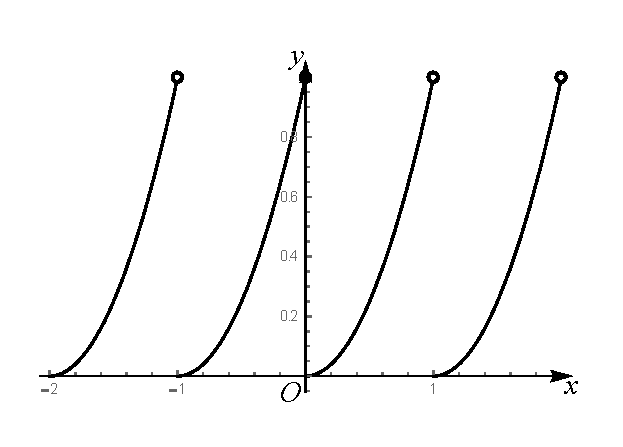
\includegraphics[height=0.3\textheight]{F:/life/2018AutumnTA/Exercises/1/problem8.pdf}
\end{center}
\caption{8.题$f(x)$的图像}
\end{figure}
\item[\bf9.]若已知函数$y=f(x)(-\infty<x<+\infty)$的图形, 试画出$y=f(x-a),\ y=f(ax),\ y=f(x)-a,\ y=af(x)$的图形(自己举一个具体的例子).
\newline
{\bf(口诀: 左加右减, 上加下减; 对于x, 大于1缩小, 小于1放大;  对于y, 大于1放大, 小于1缩小. 也可直观理解.)}
\newline
解:取$f(x)=\sin x,\ a=2.5$.
\begin{figure}[H]
\begin{center}
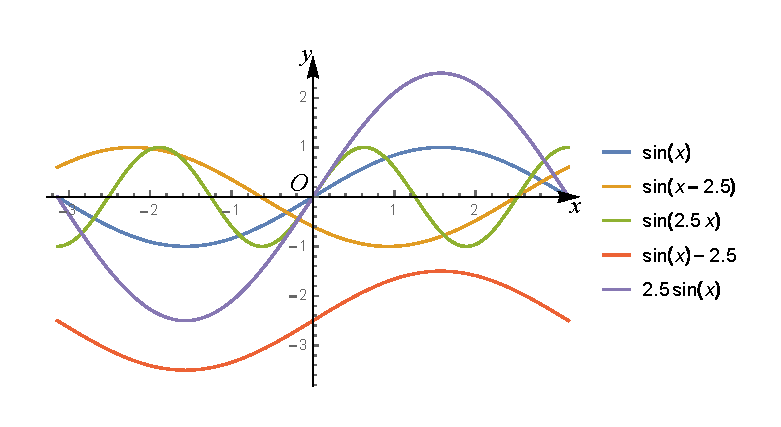
\includegraphics[height=0.3\textheight]{F:/life/2018AutumnTA/Exercises/1/problem9.pdf}
\end{center}
\caption{9.题$f(x)$的图像}
\end{figure}
\item[10.]设$f(x)=\begin{cases}x^2,&x\geq0\\-x^2,&x<0\end{cases}$,试证$f$是$\mathbb R\rightarrow\mathbb R$的一个双射, 并求它的逆映射.
\newline
{\bf(如果$f$既是单射又是满射, 则是双射. 求逆映射就是求反函数. 此题可不讲.)}
\newline
证明: 不妨设$x_1<x_2$, 可分以下三种情况讨论:
\begin{enumerate}
\item[i.]$x_1<x_2\leq0$, 此时$f(x)=-x^2$单调增加, 故$f(x_1)<f(x_2)$;
\item[ii.]$x_1\leq0<x_2$, 此时$f(x_1)\leq0<f(x_2)$;
\item[iii.]$0\leq x_1<x_2$, 此时$f(x)=x^2$单调增加, 故$f(x_1)<f(x_2)$. 
\end{enumerate}
可知$f$是$\mathbb R\rightarrow\mathbb R$的一个单射, 且$f(x)$在$(-\infty,+\infty)$上单调增加. $f(x)$的值域是$(-\infty,+\infty)=\mathbb R$, $\forall y\in\mathbb R,\ \exists x\in\mathbb R,\ \text{使得}y=f(x)$, 故$f$是$\mathbb R\rightarrow\mathbb R$的一个满射. 因此$f$是$\mathbb R\rightarrow\mathbb R$的一个双射. 其逆映射即反函数为
\[
x=\begin{cases}
\sqrt y,&y\geq0\\
\sqrt {-y},&y<0
\end{cases}.
\]
\item[\bf11.]设$f:\ X\rightarrow Y,g:\ Y\rightarrow Z$都是双射.求证$g\circ f:\ X\rightarrow Z$也是双射, 并且$(g\circ f)^{-1}=f^{-1}\circ g^{-1}$.
\newline
{\bf(双射如图所示, 单射和满射的图形也可画出.)}
\begin{figure}[H]
\begin{center}
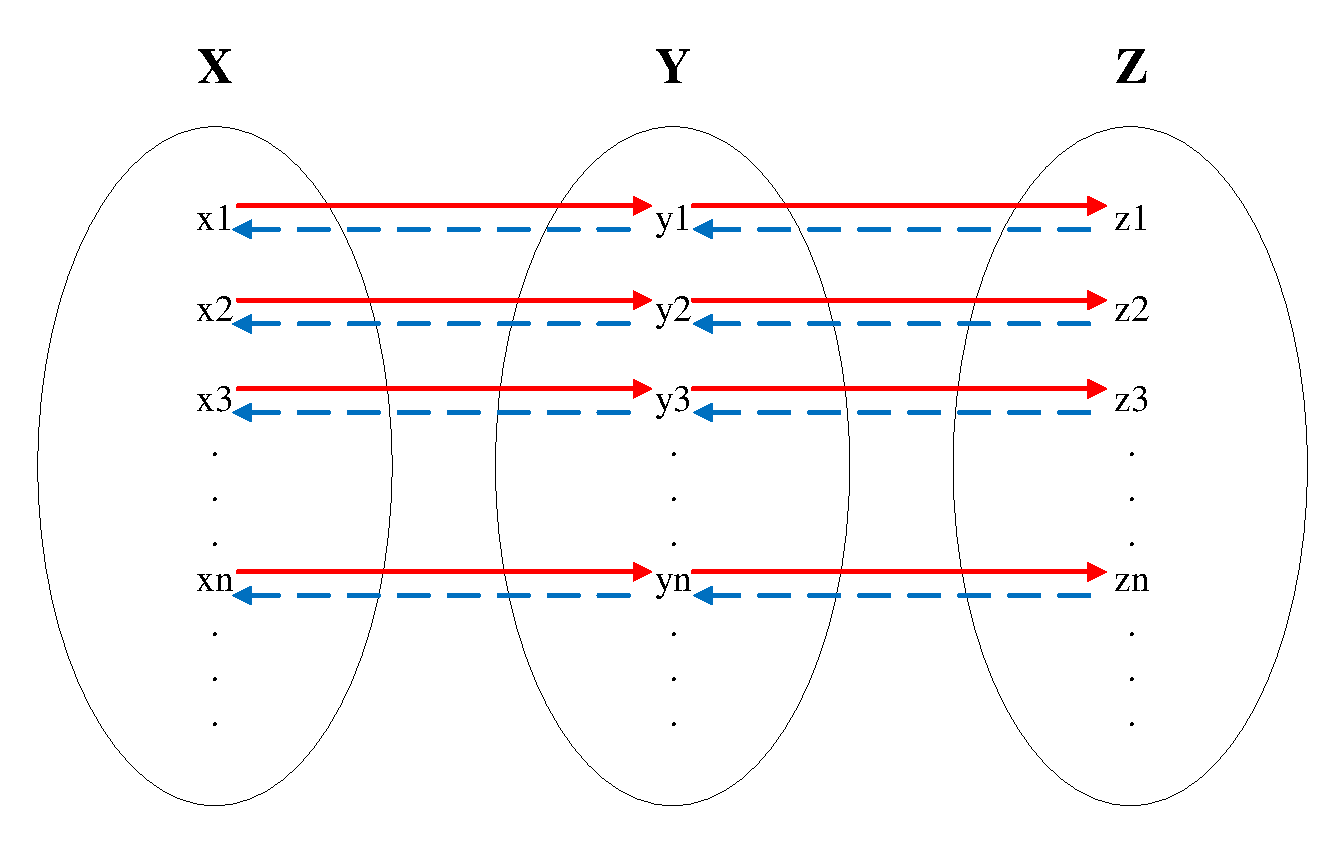
\includegraphics[height=0.3\textheight]{F:/life/2018AutumnTA/Exercises/1/problem11.pdf}
\end{center}
\caption{11.题图示}
\end{figure}


证明: $\because f:\ X\rightarrow Y,g:\ Y\rightarrow Z$都是双射, 
\newline
$\therefore \forall x\in X,\ \exists\text{唯一的} y\in Y,\ \text{满足}y=f(x)$, 对于该$y\in Y,\ \exists\text{唯一的} z\in Z,\ \text{满足}z=g(y)=g(f(x))=g\circ f(x)$; $\forall z\in Z,\ \exists\text{唯一的} y\in Y,\ \text{满足}z=g(y)$, 即$y=g^{-1}(z)$, 对于该$y\in Y,\ \exists\text{唯一的} x\in X,\ \text{满足}y=f(x)$和$z=g(y)=g(f(x))=g\circ f(x)$, 即$x=(g\circ f)^{-1}(z)=f^{-1}(y)=f^{-1}(g^{-1}(z))=f^{-1}\circ g^{-1}(z)$. 
\newline
$\therefore g\circ f:\ X\rightarrow Z$是双射, 且$(g\circ f)^{-1}=f^{-1}\circ g^{-1}$.
\newline
{\bf(结合图示说明.)}
\item[\bf12.]试写出一个从$(0,1)$到$(-\infty,+\infty)$的双射; 写出一个自然数集到整数集的双射.
\newline
解:(1)$y=\cot\pi x,\ 0<x<1$或$y=\tan\pi(x-\frac12),\ 0<x<1${\bf(先伸缩后平移)};
\newline
(2){\bf(构造)}$y=\begin{cases}
k,&x=2k\\
0,&x=0\\
-k,&x=2k-1
\end{cases},x\in\mathbb Z/\mathbb Z^-$.
\end{enumerate}
\subsection{初等函数与非初等函数}
\noindent
\subsubsection{知识结构}
\noindent第一章实数与函数
	\begin{enumerate}
		\item[1.1] 集合与符号
		\item[1.2] 实数和实数集
		\item[1.3] 函数
		\item[1.4] 初等函数
			\begin{itemize}
				\item能用公式表示的函数有两大类:
					\begin{itemize}
						\item初等函数
						\item非初等函数
					\end{itemize}
				\item基本初等函数
					\begin{enumerate}
						\item[1.]常值函数
						\item[2.]幂函数
						\item[3.]指数函数
						\item[4.]对数函数
						\item[5.]三角函数
						\item[6.]反三角函数
					\end{enumerate}
				\item初等函数: 基本初等函数经过有限次四则运算和有限次复合所得到的函数称为初等函数.
					\begin{enumerate}
						\item[7.]双曲函数
					\end{enumerate}
			\end{itemize}
			\item[1.5] 非初等函数: 分段函数、隐函数、用参数式确定的函数, 以及用积分和级数表示的函数等
				\begin{enumerate}
					\item[1.5.1]分段函数
						\begin{itemize}
							\item符号函数
							\item取整函数
						\end{itemize}
					\item[1.5.2]其他非初等函数(隐函数)
						\begin{itemize}
							\item螺线
							\item旋轮线
						\end{itemize}					
				\end{enumerate}
	\end{enumerate}
\subsubsection{双曲正弦}
\begin{enumerate}
	\item双曲正弦$\Rightarrow$反双曲正弦
	\item反双曲正弦$\Rightarrow$双曲正弦, 即习题3
\end{enumerate}
\subsubsection{习题1.4解答}
\begin{enumerate}
\item 求下列函数的定义域:
\newline
$(1)y=\sqrt{x^2-x}\cdot\arcsin x;\hspace{3cm}(2)y=\lg(\lg(\lg x));$
\newline
$(3)y=\arccos e^{2x};\hspace{4.5cm}{\bf(4)}y=\sqrt{\lg(x^2-1)}.$
\newline
{\bf(定义域应写成集合或区间.)}
\newline
解:(1)$y=\sqrt{x^2-x}\cdot\arcsin x,\ \Rightarrow x^2-x\geq0\text{且}-1\leq x\leq1,\ \Rightarrow x(x-1)\geq0\text{且}-1\leq x\leq1,\ \Rightarrow x\geq1\text{或}x\leq0,\text{且}-1\leq x\leq1,\ \Rightarrow x=1\text{或}-1\leq x\leq0,\ \Rightarrow$ 定义域为$[-1,0]\cup\{1\}$.
\newline
(2)$y=\lg(\lg(\lg x)),\ \Rightarrow x>0\text{且}\lg x>0\text{且}\lg(\lg x)>0,\ \Rightarrow x>0\text{且}x>1\text{且}\lg x>1,\ \Rightarrow x>0\text{且}x>1\text{且}x>10,\ \Rightarrow x>10,\ \Rightarrow$ 定义域为$(10,+\infty)$.
\newline
(3)$y=\arccos e^{2x},\ \Rightarrow -1\leq e^{2x}\leq1,\ \Rightarrow 2x\leq0,\ \Rightarrow x\leq0,\ \Rightarrow$ 定义域为$(-\infty,0]$.
\newline
{\bf(4)}$y=\sqrt{\lg(x^2-1)},\ \Rightarrow x^2-1>0\text{且}\lg(x^2-1)>0,\ \Rightarrow x>1\text{或}x<-1,\ \text{且}x^2-1>1,\ \Rightarrow x>1\text{或}x<-1,\ \text{且}x>\sqrt2\text{或}x<-\sqrt2,\ \Rightarrow x>\sqrt2\text{或}x<-\sqrt2,\ \Rightarrow$ 定义域为$(-\infty,\sqrt2)\cup(\sqrt2,+\infty)$.
\item设$f(x)$是定义在$(-\infty,+\infty)$上的奇函数, 在$(0,+\infty)$上的表达式为$f(x)=x-x^2$. 求$f(x)$在$(-\infty,0)$上的表达式.
\newline
解: 当$x<0$时,$f(x)=-f(-x)=-(-x)+(-x)^2=x+x^2.$
\item[\bf3.]验证$y=\ln(\sqrt{x^2+1}+x)$是奇函数, 求这个函数的反函数.
\newline
解: $y(-x)=\ln(\sqrt{x^2+1}-x)=-\ln\frac1{\sqrt{x^2+1}-x}=-\ln\frac{\sqrt{x^2+1}+x}{x^2+1-x^2}=-\ln(\sqrt{x^2+1}+x)=-y(x)$, 故$y=\ln(\sqrt{x^2+1}+x)$是奇函数.
\newline
由$y=\ln(\sqrt{x^2+1}+x)$得$e^y=\sqrt{x^2+1}+x$(*), 由$y(x)=-y(-x)=-\ln(\sqrt{x^2+1}-x)$得$e^{-y}=\sqrt{x^2+1}-x$(**). (*)式和(**)相减可得$x=\frac{e^y-e^{-y}}2$. 反函数为$y=\frac{e^x-e^{-x}}2$.
\item[\bf4.]设$f(x)$是定义在$(-\infty,+\infty)$的函数. 对于任意两个实数$x,y$, 满足$f(x+y)=f(x)+f(y)$. 求证存在常数$a$, 使得对于所有的有理数$x$, 都有$f(x)=ax$.
\newline
{\bf(此题较难, 可不讲.)}
\newline
证明: $\because\forall x,y\in\mathbb R,f(x+y)=f(x)+f(y),\ \therefore f(0)=f(0)+f(0)=0,\ f(x-x)=f(x)+f(-x)=f(0)=0,\ \therefore f(x)=-f(-x),\ \therefore f(x)$是奇函数, 因此只需证明$x>0$的情况. 
\newline
当$x=n,\ n\in\mathbb Z^+$时, $f(2)=f(1)+f(1)=2f(1),\ f(3)=f(2)+f(1)=3f(1),\dots,\ f(n)=nf(1),\dots$, 即$f(x)=f(1)x$;
\newline
当$x=\frac1n,\ n\in\mathbb Z^+$时, $f(1)=f(\frac1n)+f(\frac{n-1}n)=2f(\frac1n)+f(\frac{n-2}n)=\dots=nf(\frac1n),\ \therefore f(\frac1n)=\frac1nf(1)$, 即$f(x)=f(1)x$;
\newline
当$x=\frac mn,\ m,n\in\mathbb Z^+$时, $f(\frac mn)=f(\frac1n)+f(\frac{m-1}n)=mf(\frac1n)=\frac mnf(1)$, 即$f(x)=f(1)x$.
\newline
综上所述, 存在常数$a=f(1)$使得对于所有的有理数x, 都有$f(x)=ax$.
\end{enumerate}
\subsection{补充内容}
维基百科是重要的工具, 上面有各种总结得很好的内容, 可以经常浏览, 拓展知识面. 比如:
\begin{itemize}
	\item 三角函数 \url{https://en.wikipedia.org/wiki/Trigonometric_functions}
	\item 双曲函数 \url{https://en.wikipedia.org/wiki/Hyperbolic_function}
	\item 雅可比椭圆函数 \url{https://en.wikipedia.org/wiki/Jacobi_elliptic_functions}
\end{itemize}
\end{document}